\documentclass[11pt,a4paper]{article}
\usepackage[margin=2.4cm]{geometry}
\usepackage{amsmath,amssymb}
\usepackage{booktabs}
\usepackage{graphicx}
\usepackage{xcolor}
\usepackage[colorlinks=true,linkcolor=blue!50!black,urlcolor=blue!50!black,
            citecolor=blue!50!black]{hyperref}
\usepackage{caption}
\captionsetup{font=small}

\newcommand{\xB}{x_{\mathrm{B}}}
\newcommand{\Ein}{E_{\mu}}
\newcommand{\Eout}{E_{\mu'}}
\newcommand{\Ehad}{E_{\mathrm{had}}}
\newcommand{\thmu}{\theta_{\mu}}
\newcommand{\thh}{\theta_{h}}
\newcommand{\GeV}{\,\mathrm{GeV}}
\newcommand{\fb}{\,\mathrm{fb}^{-1}}
\newcommand{\note}[1]{\textcolor{red}{\textbf{#1}}}

\title{\bf Charm production in muon deep-inelastic scattering with FASER\emph{Cal}\\[4pt]
\large Yields, charm/anticharm tagging, and Bjorken-$x$ reconstruction}
\author{Internal note --- generated from the \texttt{muondis-fasercal} analysis}
\date{\today}

\begin{document}
\maketitle

\begin{abstract}
\noindent
We study charm production in high-energy muon deep-inelastic scattering (DIS) in
FASER\emph{Cal}, using the POWHEG\,+\,Pythia8 muon-DIS samples developed for the
FASER$\nu$ programme, and the FASER\emph{Cal} geometry and detector performance
as given in the Conceptual Design Report and the July 2026 collaboration-meeting
talk. Three results. First, the charm/anticharm asymmetry $A_c$ --- the
observable that originally motivated the study --- is \emph{identically zero} in
the available PDF sets, so it cannot be used as an intrinsic-charm observable
without a PDF set carrying an explicit charm asymmetry. Second, the accessible
intrinsic-charm signal is instead the large-$\xB$ charm excess, and we confirm
that the lepton-only $\xB$ reconstruction used in the literature is destroyed by
FASER\emph{Cal}'s muon-momentum resolution. Third, and centrally, we show that
\emph{calorimetric} reconstruction methods --- which FASER$\nu$ cannot use ---
recover a factor $\sim\!3$--$3.8$ of the large-$\xB$ signal, and raise the
intrinsic-charm purity of the selected sample from $64\%$ to $95\%$ when two
statistically independent methods are combined. All uncertainties quoted are
statistical and detector-resolution effects only; systematic uncertainties are
discussed in Sec.~\ref{sec:syst} but are \emph{not} included in any number.
\end{abstract}

\tableofcontents

%======================================================================
\section{Motivation and scope}

The proton may carry a non-perturbative, ``intrinsic'' charm (IC) component: a
$|uudc\bar{c}\rangle$ Fock state in which the charm quarks carry a large fraction
of the proton momentum. Its signature is an excess of charm at large Bjorken
$\xB$ over what perturbative gluon splitting produces. High-energy muon DIS at
the LHC is a clean probe, and FASER\emph{Cal} --- an electronic, highly
segmented three-dimensional scintillator calorimeter with a downstream
magnetised muon spectrometer --- is a candidate detector.

This note addresses three questions:
\begin{enumerate}
  \item How many muon-DIS charm events does FASER\emph{Cal} collect, and can
        charm be distinguished from anticharm? (Sec.~\ref{sec:chain})
  \item Is the charm/anticharm asymmetry $A_c$ a usable intrinsic-charm
        observable? (Sec.~\ref{sec:asym})
  \item Can $\xB$ be reconstructed well enough at large $\xB$ for the
        intrinsic-charm excess to survive? (Sec.~\ref{sec:xreco})
\end{enumerate}

The third is the critical one. Ref.~\cite{francener} reconstructs $\xB$ from the
scattered muon alone and finds that a muon-momentum smearing of $10\%$ already
reduces the $\xB\!\geq\!0.2$ charm excess from ${\times}8$ to ${\times}2$, and
that $30\%$ removes it entirely. FASER\emph{Cal}'s spectrometer is iron-core and
multiple-scattering dominated, so this is a genuine threat --- but FASER\emph{Cal}
is also a calorimeter, which FASER$\nu$ is not.

%======================================================================
\section{Inputs and their provenance}
\label{sec:inputs}

Every number used is listed in Table~\ref{tab:inputs} with its source. Where a
quantity is an assumption rather than a documented value, this is stated
explicitly; those are the entries that most need review.

\begin{table}[htbp]
\centering\small
\begin{tabular}{lll}
\toprule
Quantity & Value & Source \\
\midrule
Run 4 luminosity & $780\fb$ & FASER\emph{Cal} talk; CDR Sec.~3.1 \\
3DCal geometry & 10 modules $\times$ 20 layers of $1\,$cm$^3$ cubes & talk slide 4 \\
3DCal transverse face & $48\times48\,$cm$^2$ & talk slide 11 \\
Tungsten absorber & 1, 5 or 10\,mm \emph{per module} & talk slide 39; CDR Table 5 \\
3DCal total mass & 581 / 896 / 1118\,kg & CDR Table 5 \\
Fiducial region & $z<1150\,$mm ($48\%$ of length) & CDR Table 8 \\
Position & LoS shift $(452,236)\,$mm, tilt $4.5^\circ$ & talk slides 11--12 \\
Muon momentum resolution & $20/22.8/29/63.1\%$ at $20/100/200/1000\GeV$ & CDR Sec.~2.6.2 \\
Charge misidentification & $<0.7\%$ below $100\GeV$; $2$--$5\%$ at TeV & CDR Sec.~2.6.2 \\
Spectrometer acceptance & $43\%$ ($\geq2$ MDT stations) & talk slide 33 \\
Hadronic energy resolution & $\sim 9\%$ & talk (\,$p_{\rm jet}$, NC\,) \\
\midrule
Off-axis flux factor & $F_{\rm flux}=0.96$ & \emph{this work}, from FLUKA \\
Run 4 optics enhancement & $F_{\rm optics}=2.0$ & CDR Sec.~1.3.2 (rate $\times2$) \\
Muon angular resolution & $0.3\,$mrad & \emph{derived} from 3DCal geometry \\
Hadronic angular resolution & $20\,$mrad & \note{ASSUMPTION -- no source} \\
Identification\,+\,linking eff. & scanned $0.05$--$1$ & \note{not assumed; scanned} \\
\bottomrule
\end{tabular}
\caption{Inputs. Entries above the rule are taken from FASER\emph{Cal}
documents; below the rule are derived or assumed in this work. Where the talk
and the CDR disagree, the talk (more recent) is used.}
\label{tab:inputs}
\end{table}

\subsection{Monte Carlo samples}
Two POWHEG\,+\,Pythia8 productions differing \emph{only} in the charm PDF:
\begin{center}\small
\begin{tabular}{lll}
\toprule
Production & LHAPDF & Role \\
\midrule
\texttt{production\_v1} & 331100, \texttt{NNPDF40\_nnlo\_as\_01180} & fitted charm (IC allowed) \\
\texttt{production\_pc} & 332100, \texttt{NNPDF40\_nnlo\_pch\_as\_01180} & perturbative charm (null) \\
\bottomrule
\end{tabular}
\end{center}
Muon beam on a fixed nucleon target, $Q_{\min}=1.65\GeV$, four per-nucleon
samples ($\mu^\pm$ on $p/n$). 25 independent seeds, $1.90\times10^{6}$ showered
events per hypothesis. The muon flux is implemented as a beam PDF of a
fictitious $7\,\mathrm{TeV}$ beam~\cite{francener}; this has consequences discussed in
Sec.~\ref{sec:hadsys}.

Target composition is applied at analysis time: FASER\emph{Cal} is polystyrene
(CH, $w_p=0.538$) plus tungsten ($w_p=0.402$), not the tungsten-only target of
FASER$\nu$.

%======================================================================
\section{The muon-DIS charm chain}
\label{sec:chain}

\subsection{Charm tagging without a vertex}
In emulsion, charm is identified by imaging the sub-mm decay kink. In a
scintillator this is impossible: the charm flight length is a few mm, at or
below cell size, and in the interleaved-tungsten configuration the decay happens
inside an absorber plate. \textbf{There is no displaced-vertex charm tag in
FASER\emph{Cal}.}

The surviving handle is the muon from the semileptonic charm decay, whose charge
\emph{is} the charm sign:
\begin{equation}
  c \to s\,W^+,\; W^+\!\to\mu^+\nu \qquad
  \bar{c} \to \bar{s}\,W^-,\; W^-\!\to\mu^-\bar{\nu}.
\end{equation}
This gives an opposite-sign dimuon: the scattered DIS muon plus a softer muon of
opposite charge. FASER\emph{Cal} itself has no field; the sign comes from the
downstream spectrometer. The identity $\mathrm{sign}(c)=q_\mu$ is verified
event-by-event in the code and holds for $100\%$ of events.

\subsection{Yields}
Table~\ref{tab:chain} gives the chain at Run 4 nominal conditions.

\begin{table}[htbp]
\centering\small
\begin{tabular}{lrrr}
\toprule
Stage & 3DCal only & $+$AHCAL & Fraction \\
\midrule
Muon DIS in fiducial volume & 373\,601 & 2\,503\,837 & $100\%$ \\
\quad containing charm & 10\,578 & 71\,489 & $2.86\%$ \\
\quad charm $\to$ semileptonic $\mu$ & 1\,866 & 12\,613 & $17.6\%$ of charm \\
\quad $\mu$ punches out of calorimeter & 1\,523 & 10\,301 & $81.7\%$ \\
\quad reaches spectrometer ($43\%$) & 666 & 4\,509 & $43\%$ \\
\quad identified $+$ linked ($\varepsilon=0.9$) & \textbf{599} & \textbf{4\,058} & $0.16\%$ of DIS \\
\midrule
Charge-tag purity & \multicolumn{2}{c}{$99.1\%$} & CDR Sec.~2.6.2 \\
Statistical reach $\sigma(A_c)$ & $0.041$ & $0.016$ & \\
\bottomrule
\end{tabular}
\caption{Muon-DIS charm chain, Run 4 ($780\fb$), 3DCal with 1\,mm W per module,
fiducial $z<1150\,$mm ($277\,$kg), $F_{\rm flux}=0.96$, $F_{\rm optics}=2.0$.}
\label{tab:chain}
\end{table}

Two features dominate. The chain is \textbf{branching-limited, not
detector-limited}: $2.86\%\times17.6\%\approx1/200$ before any detector effect,
and no instrumentation improvement recovers it. And $94\%$ of charm events
contain \emph{two} charm hadrons --- the signature of photon-gluon fusion
$\gamma g\to c\bar{c}$ --- which is why the per-event semileptonic rate
($17.6\%$) is about twice the per-hadron branching ratio.

Acceptance is an \emph{angular} problem, not a momentum one: the decay muon has a
median angle of $33\,$mrad against the scattered muon's $4.3\,$mrad, and $83\%$
already pass the punch-through momentum threshold. The assumed $43\%$ acceptance
corresponds to a $\theta<8.7\,$mrad cone. Charge identification is
\emph{not} a bottleneck: with a median decay-muon momentum of $11.5\GeV$, the
CDR misidentification is $<0.7\%$.

\subsection{Absorber and AHCAL options}
\begin{center}\small
\begin{tabular}{lrrr}
\toprule
Configuration & Fiducial mass & Tagged & $\sigma(A_c)$ \\
\midrule
1\,mm W / module (baseline) & 277\,kg & 599 & 0.041 \\
5\,mm W / module & 421\,kg & 901 & 0.033 \\
10\,mm W / module & 514\,kg & 1102 & 0.030 \\
$+$ AHCAL (1.60\,t fiducial, $\sim\!98\%$ Fe) & 1\,877\,kg & 4\,058 & 0.016 \\
\bottomrule
\end{tabular}
\end{center}
The AHCAL adds $5.8\times$ the 3DCal target mass. Its $4\times4\,$cm$^2$
granularity makes vertex finding and muon linking harder, so its curve should be
read at a \emph{lower} identification efficiency --- which is why the main
result is presented against $\varepsilon$ rather than at a fixed value.

%======================================================================
\section{The charm/anticharm asymmetry is not a usable observable}
\label{sec:asym}

\subsection{It is zero by construction}
Direct inspection of the LHAPDF grids gives, at $Q=10\GeV$:
\begin{center}\small
\begin{tabular}{lrrr}
\toprule
$x$ & $x c(x)$ & $x\bar{c}(x)$ & $(c-\bar{c})/(c+\bar{c})$ \\
\midrule
0.01 & $2.043\times10^{-1}$ & $2.047\times10^{-1}$ & $-1.0\times10^{-3}$ \\
0.30 & $8.635\times10^{-3}$ & $8.669\times10^{-3}$ & $-2.0\times10^{-3}$ \\
0.70 & $5.190\times10^{-4}$ & $5.191\times10^{-4}$ & $-7.3\times10^{-5}$ \\
\bottomrule
\end{tabular}
\end{center}
Over all 2352 grid points the maximum of $|c-\bar{c}|/(c+\bar{c})$ is
$6.4\times10^{-3}$, and the number sum rule gives
$\int(c-\bar{c})\,dx\,/\!\int(c+\bar{c})\,dx = -1.5\times10^{-4}$. NNPDF4.0 fits
the total $c+\bar{c}$ and sets $c-\bar{c}=0$. The residual is \emph{larger} in
the perturbative set than the fitted one --- the signature of numerical noise
rather than physics.

This is consistent with the light-cone argument: the minimal
$|uudc\bar{c}\rangle$ Fock state contains one $c$ and one $\bar{c}$ with
identical distributions, so BHPS intrinsic charm predicts $A_c(x)=0$ at every
$x$. A non-zero $A_c$ requires physics beyond the minimal Fock state, is
model-dependent, and is constrained by $\int(c-\bar{c})dx=0$.

\subsection{But fragmentation generates one}
Even with an exactly symmetric charm PDF, the \emph{observable} sample is
asymmetric, through the leading-baryon effect:
\begin{center}\small
\begin{tabular}{lrrrr}
\toprule
Species & $N(c)$ & $N(\bar{c})$ & Ratio & BR$(\to\mu)$ \\
\midrule
$\Lambda_c$ & 13\,430 & 1\,963 & \textbf{6.84} & $4.8\%$ \\
$D^+$ & 16\,683 & 20\,355 & 0.82 & $16.7\%$ \\
$D^0$ & 31\,730 & 38\,820 & 0.82 & $6.6\%$ \\
\bottomrule
\end{tabular}
\end{center}
The $c$ quark can pick up two valence quarks from the target remnant to form a
$\Lambda_c$; the $\bar{c}$ cannot easily form an antibaryon. $\Lambda_c$ also has
the lowest semileptonic branching ratio of any charm hadron, so the $c$ is
preferentially \emph{hidden from the muon tag} while the $\bar{c}$ is not,
leaving a $\bar{c}$-enriched tagged sample: $A=-0.061\pm0.036$
($N_{\rm eff}=778$, i.e.\ $1.7\sigma$).

\paragraph{Consequences.} $A_c$ cannot be used as an IC observable with existing
PDF inputs, and the fragmentation-induced asymmetry is of the \emph{same size} as
our statistical reach ($0.041$), so it is a competing background rather than a
correction. Attention should move to the large-$\xB$ excess.

\subsection{The signal that does exist}
The fitted/perturbative charm ratio at $Q=10\GeV$:
\begin{center}\small
\begin{tabular}{lrrrrr}
\toprule
$x$ & 0.2 & 0.3 & 0.4 & 0.5 & 0.7 \\
\midrule
fitted / perturbative & $1.8$ & $3.2$ & $5.7$ & $10.9$ & $44.3$ \\
\bottomrule
\end{tabular}
\end{center}
At \emph{event} level, integrated above $\xB=0.2$, the charm sample is
$\approx99\%$ IC-attributable (Sec.~\ref{sec:icfrac}).

%======================================================================
\section{Bjorken-$x$ reconstruction}
\label{sec:xreco}

\subsection{Kinematics and notation}
For fixed-target DIS with nucleon mass $M$, incoming muon energy $\Ein$,
scattered muon energy $\Eout$ and scattering angle $\thmu$:
\begin{equation}
  \nu = \Ein - \Eout, \qquad
  Q^2 = 2\Ein\Eout(1-\cos\thmu), \qquad
  \xB = \frac{Q^2}{2M\nu}, \qquad y=\frac{\nu}{\Ein}.
\end{equation}
The hadronic system recoiling against the muon is exactly $X=q+p_{\rm target}$,
so it is fully determined by the muon kinematics:
\begin{equation}
  \Ehad = \nu + M,\qquad
  p_T^{\rm had} = \Eout\sin\thmu,\qquad
  p_z^{\rm had} = |p_\mu| - \Eout\cos\thmu .
  \label{eq:hadcons}
\end{equation}

The key numbers of the problem, from our sample:
\begin{center}\small
\begin{tabular}{lr}
\toprule
Median $\Ein$ & $665\GeV$ \\
Median $\Eout$ & $469\GeV$ \\
Median $\nu$ & $52\GeV$ \\
Median $y$ & $0.161$ \\
Median $\thmu$ & $4.3\,$mrad \\
Median $\thh$ & $81\,$mrad \\
\bottomrule
\end{tabular}
\end{center}
\textbf{$\nu$ is only $7.7\%$ of $\Ein$.} It is a small difference of two large
numbers, and this single fact drives everything that follows.

%----------------------------------------------------------------------
\subsection{Method 1: lepton-only}
\label{sec:lepton}

\paragraph{What it does.} Uses only the muon. Both muon energies and the
scattering angle are measured; $\nu$ and $Q^2$ follow directly:
\begin{equation}
  \nu^{\rm lep} = \Ein - \Eout,\qquad
  Q^2_{\rm lep} = 2\Ein\Eout(1-\cos\thmu),\qquad
  x_{\rm lep} = \frac{Q^2_{\rm lep}}{2M\nu^{\rm lep}} .
\end{equation}

\paragraph{Why it is used.} It is the only method available to an emulsion
detector. FASER$\nu$ measures angles superbly and energy not at all, so it is
\emph{forced} into this choice. It is what Ref.~\cite{francener} uses.

\paragraph{Why it fails here.} Because $\nu$ is a difference of two large
numbers, a fractional error $\epsilon$ on each muon leg propagates as
\begin{equation}
  \frac{\sigma_\nu}{\nu} \;\approx\; \frac{\epsilon}{y}\sqrt{1+(1-y)^2}
  \;\sim\; \frac{\epsilon}{y} .
\end{equation}
With $y=0.16$ and the CDR resolution $\sigma_p/p\approx38\%$ at $469\GeV$, this
gives a \emph{several-hundred-percent} error on $\nu$. Measured directly, the
$\nu$ resolution is an interquartile range of $410\%$. The migration matrix
(Fig.~\ref{fig:migration}) shows essentially \emph{no} correlation between
$x_{\rm true}$ and $x_{\rm reco}$.

\paragraph{Additional problem.} It requires $\Ein$. The downstream spectrometer
sees only the \emph{outgoing} muon, so if the incoming muon is not measured
elsewhere this method \textbf{does not exist at all}.

%----------------------------------------------------------------------
\subsection{Method 2: Jacquet--Blondel}
\label{sec:jb}

\paragraph{What it does.} Uses only the \emph{hadronic} system. The energy
transfer is measured directly by the calorimeter rather than inferred from a
difference:
\begin{equation}
  \nu^{\rm JB} = \Ehad - M,\qquad
  Q^2_{\rm JB} = \frac{(p_T^{\rm had})^2}{1-y},\qquad
  x_{\rm JB} = \frac{Q^2_{\rm JB}}{2M\nu^{\rm JB}} .
\end{equation}

\paragraph{Why the target-mass subtraction matters.} The measured hadronic energy
is $\nu+M$ (Eq.~\ref{eq:hadcons}); it includes the struck nucleon's rest energy.
Omitting $M$ biases $x_{\rm JB}$ low by $M/\nu$, which is $9\%$ on the
$\xB\geq0.2$ sample where $\nu\approx9\GeV$. This is a small but real effect that
is easy to miss.

\paragraph{Strengths.} The muon momentum is not used \emph{at all}: a $9\%$
hadronic resolution gives a $9\%$ error on $\nu$, not an amplified one. $\Ein$
enters only through the mild $(1-y)$ factor, so the method survives when $\Ein$
is unmeasured.

\paragraph{Weaknesses.} $Q^2$ comes from the hadronic transverse momentum, which
is the \emph{difference} of a nearly-forward system --- so it is sensitive to the
hadronic \emph{angular} resolution. In practice JB has excellent efficiency
($78\%$) but poor purity ($34\%$): the vastly more numerous low-$\xB$ events
migrate upward and flood the selection.

%----------------------------------------------------------------------
\subsection{Method 3: the $\Sigma$ method}
\label{sec:sigma}

\paragraph{The idea.} Reconstruct the \emph{incoming} muon energy from the final
state, so that it need not be measured. With the beam along $+z$, the initial
state has $E+p_z = 2\Ein + M$, and since $E+p_z$ is conserved,
\begin{equation}
  2\Ein \;=\; \sum_{\rm had}(E+p_z) \;+\; \Eout(1+\cos\thmu) \;-\; M ,
  \label{eq:sigma}
\end{equation}
after which one proceeds exactly as in the lepton-only method but with this
$\Ein$.

\paragraph{A necessary derivation.} The collider $\Sigma$ method uses
$E-p_z$~\cite{bassler}. For a \emph{fixed target} with the beam along $+z$ that
combination is identically $M$ for the initial state and therefore carries no
information. The correct fixed-target analogue uses $E+p_z$, as in
Eq.~\ref{eq:sigma}. This was derived for this work.

\paragraph{Why it works --- an exact cancellation.} At the small angles relevant
here, $E+p_z\approx 2E$, and Eq.~\ref{eq:sigma} reduces to simple energy
conservation, $\Ein \approx \Eout + \Ehad - M$. Then
\begin{equation}
  \boxed{\;\nu^{\Sigma} \;=\; \Ein^{\rm reco} - \Eout^{\rm reco}
  \;=\; \bigl(\Eout+\Ehad-M\bigr)-\Eout \;=\; \Ehad - M\;}
\end{equation}
\textbf{The muon-momentum error appears in both terms and cancels exactly.} The
resulting $\nu$ resolution is $13\%$ (interquartile), against $410\%$ for
lepton-only where $\Ein$ and $\Eout$ are measured independently and their errors
\emph{add}. This is an algebraic cancellation, not a tuned improvement, which is
why the method is robust.

\paragraph{Insensitivity to the hadronic angle.} $p_z = |p|\cos\thh$, and with
$\thh\approx81\,$mrad a $20\,$mrad smearing changes $\cos\thh$ by $0.2\%$. The
method is therefore \emph{first-order insensitive} to the hadronic angular
resolution --- the single largest unknown in the calorimetric methods.

\paragraph{Practical note.} A user asking ``can we measure $\Ein$ by taking the
spectrometer muon and adding the energy that went into the interaction?'' is
describing exactly this method. The two constructions are numerically identical
here.

%----------------------------------------------------------------------
\subsection{Method 4: double-angle}
\label{sec:da}

\paragraph{What it does.} Uses only the two \emph{angles}, plus the beam energy.
Solving energy--momentum conservation for the scattered muon energy:
\begin{equation}
  \Eout^{\rm DA} = \Ein\,\frac{\sin\thh}{\sin(\thmu+\thh)} ,
\end{equation}
then $Q^2$ and $\nu$ as usual. Being built from angles, it is immune to
\emph{energy-scale} errors in both the calorimeter and the spectrometer --- a
genuine advantage, since energy scales are the hardest thing to calibrate.

\paragraph{Weaknesses.} Two.
\begin{enumerate}
  \item It requires $\Ein$, and $x_{\rm DA}\propto\Ein$ linearly. If the incoming
        muon is not measured, the method \textbf{does not exist}.
  \item It depends entirely on the hadronic angle $\thh$, which in a calorimeter
        is a \emph{shower axis}, not a track. Its performance degrades steeply
        with $\sigma_{\thh}$ (Fig.~\ref{fig:effpur}, left): the figure of merit
        falls from $0.65$ to $0.36$ between $0$ and $50\,$mrad.
\end{enumerate}
Since $\sigma_{\thh}$ is currently an assumption with no documented value, the
double-angle numbers carry the largest modelling uncertainty of the four.

%----------------------------------------------------------------------
\subsection{Validation}
With all resolutions set to zero, all four methods return
$x_{\rm reco}/x_{\rm true}=1.0000$. The framework is therefore verified
\emph{before} any smearing is applied. This test was essential: it exposed both
the missing target-mass term in JB and a serious problem with the hadronic
energy definition (Sec.~\ref{sec:hadsys}).

%----------------------------------------------------------------------
\subsection{Results}
\label{sec:results}

The figure of merit is efficiency $\times$ purity for the $\xB\geq0.2$
selection on charm events, where
\emph{efficiency} is the fraction of true $\xB\geq0.2$ events reconstructed
above the cut, and \emph{purity} is the fraction of selected events that truly
have $\xB\geq0.2$.

\begin{table}[htbp]
\centering\small
\begin{tabular}{lrrrrr}
\toprule
Method & Efficiency & Purity & Eff.$\times$Pur. & vs lepton & IC fraction \\
\midrule
lepton-only & $23.7\%$ & $63.8\%$ & $0.151$ & --- & $82\%$ \\
Jacquet--Blondel & $78.2\%$ & $33.6\%$ & $0.262$ & $\times1.7$ & $38\%$ \\
$\Sigma$ & $77.1\%$ & $57.6\%$ & $0.444$ & $\times2.9$ & $64\%$ \\
double-angle & $82.5\%$ & $61.3\%$ & $0.506$ & $\times3.4$ & $72\%$ \\
\midrule
\textbf{$\Sigma$ AND double-angle} & $66.3\%$ & $85.7\%$ & $\mathbf{0.568}$ & $\mathbf{\times3.8}$ & $\mathbf{95\%}$ \\
all three & $54.9\%$ & $94.7\%$ & $0.520$ & $\times3.4$ & $97\%$ \\
\bottomrule
\end{tabular}
\caption{Large-$\xB$ signal retention, $\xB\geq0.2$, 25 seeds, all modelled
effects included. ``IC fraction'' is the intrinsic-charm-attributable fraction
of the selected sample, $1-N_{\rm pert}/N_{\rm fitted}$.}
\label{tab:xreco}
\end{table}

\subsection{Why combining works}
\label{sec:combine}
The methods fail for \emph{different} reasons, so their errors are not all
correlated. Correlation of $\log(x_{\rm reco}/x_{\rm true})$:
\begin{center}\small
\begin{tabular}{lrrrr}
\toprule
 & lepton & JB & $\Sigma$ & DA \\
\midrule
lepton-only & $1.00$ & $-0.03$ & $0.65$ & $-0.05$ \\
Jacquet--Blondel & $-0.03$ & $1.00$ & $-0.01$ & $\mathbf{0.94}$ \\
$\Sigma$ & $0.65$ & $-0.01$ & $1.00$ & $\mathbf{0.08}$ \\
double-angle & $-0.05$ & $0.94$ & $0.08$ & $1.00$ \\
\bottomrule
\end{tabular}
\end{center}
$\Sigma$ and double-angle are \textbf{nearly independent} ($0.08$): one is driven
by the calorimetric \emph{energy}, the other by the \emph{angles}. JB and
double-angle are redundant ($0.94$), both being hadronic-system-driven.
Requiring both members of the independent pair raises purity from $58\%$ to
$86\%$ and the IC fraction of the selected sample from $64\%$ to $95\%$.

Adding JB buys further purity but costs more efficiency than it gains. Note that
this is a crude AND of two cuts; a proper constrained kinematic fit using all
measurements with their covariances should do better still.

\paragraph{If $\Ein$ is not measured.} Double-angle and lepton-only cease to
exist. The fallback is $\Sigma$ AND Jacquet--Blondel (correlation $-0.01$, also
independent): efficiency $60.8\%$, purity $84.5\%$, product $0.514$ --- still
$\times3.4$ over lepton-only. $\Sigma$ alone is unchanged at $0.444$.

\subsection{Intrinsic-charm content of the selection}
\label{sec:icfrac}
At truth level the $\xB\geq0.2$ cut is well placed:
\begin{center}\small
\begin{tabular}{lrrrr}
\toprule
$x$ bin & 0.1--0.2 & 0.2--0.3 & 0.3--0.4 & $>0.4$ \\
\midrule
IC fraction & $85\%$ & $98\%$ & $99\%$ & $\sim100\%$ \\
\bottomrule
\end{tabular}
\end{center}
Integrated above $0.2$ it is $\approx99\%$. What is actually \emph{selected} is
diluted by migration from low $\xB$, where there is no IC --- this is the purity
restated in physics terms, and it is why the method combination matters
(Table~\ref{tab:xreco}, last column).

\note{Caveat:} the perturbative sample above $\xB=0.2$ has $N_{\rm eff}=7$ (966
raw events, one carrying $9\%$ of the weight). The $99\%$ survives only because
the perturbative contribution is small to begin with; the perturbative
\emph{yield} itself must not be quoted, and any ratio-based statement there
needs a dedicated high-statistics \texttt{production\_pc}.

\begin{figure}[htbp]
\centering
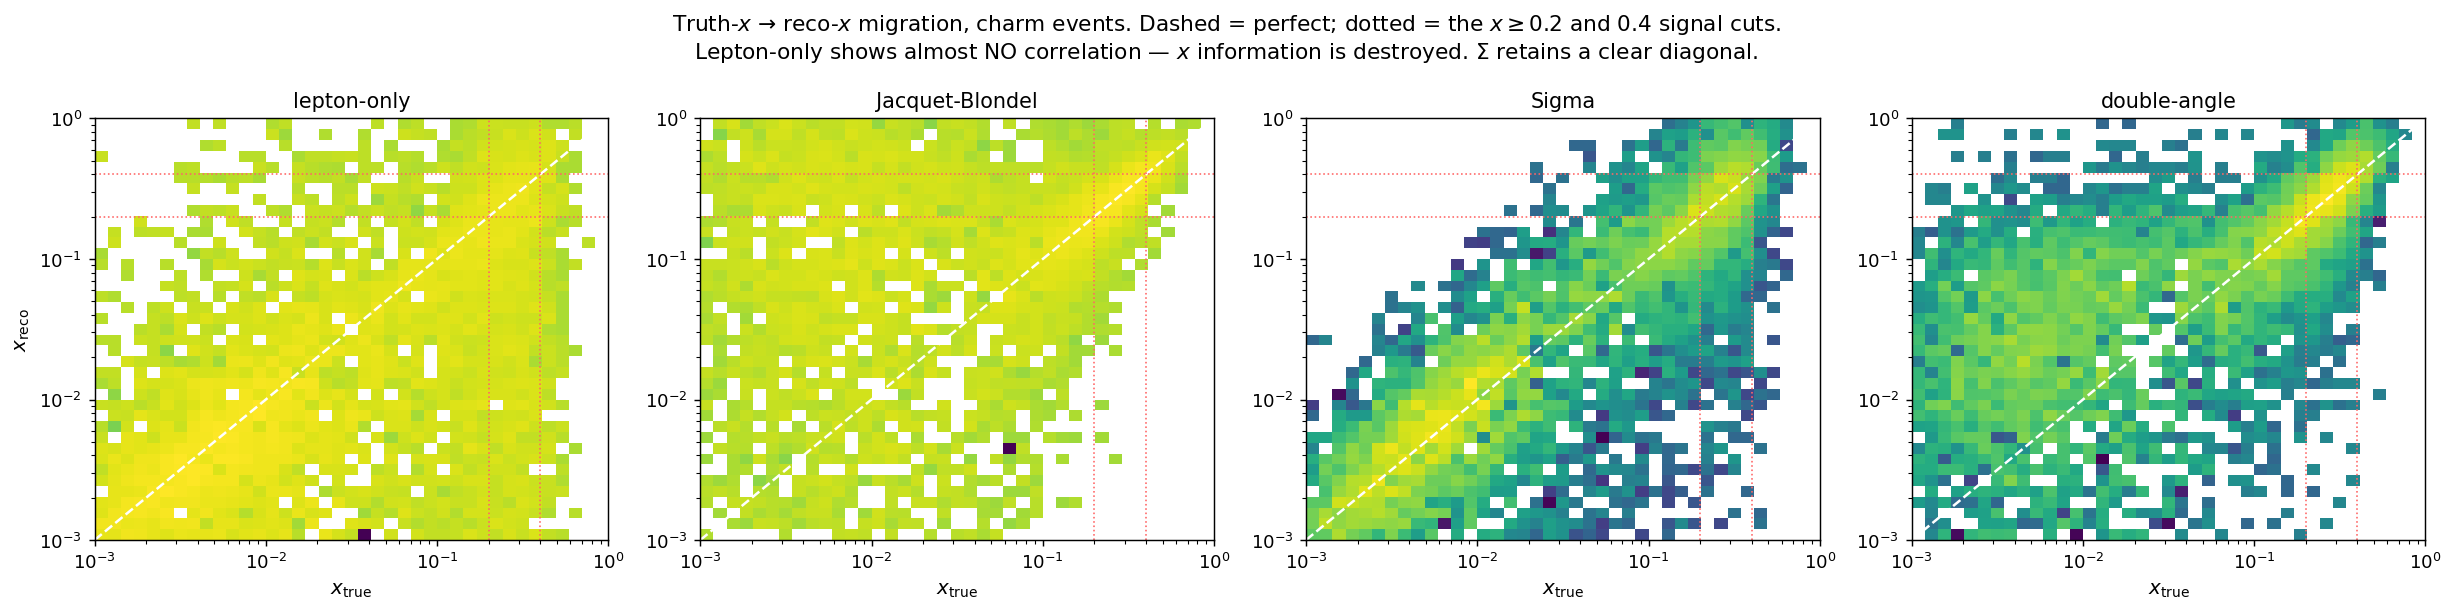
\includegraphics[width=\textwidth]{../docs/figures/30_migration.png}
\caption{Truth-$\xB$ $\to$ reco-$\xB$ migration for charm events. Dashed line is
perfect reconstruction. Lepton-only shows almost no correlation; $\Sigma$
retains a clear diagonal.}
\label{fig:migration}
\end{figure}

\begin{figure}[htbp]
\centering
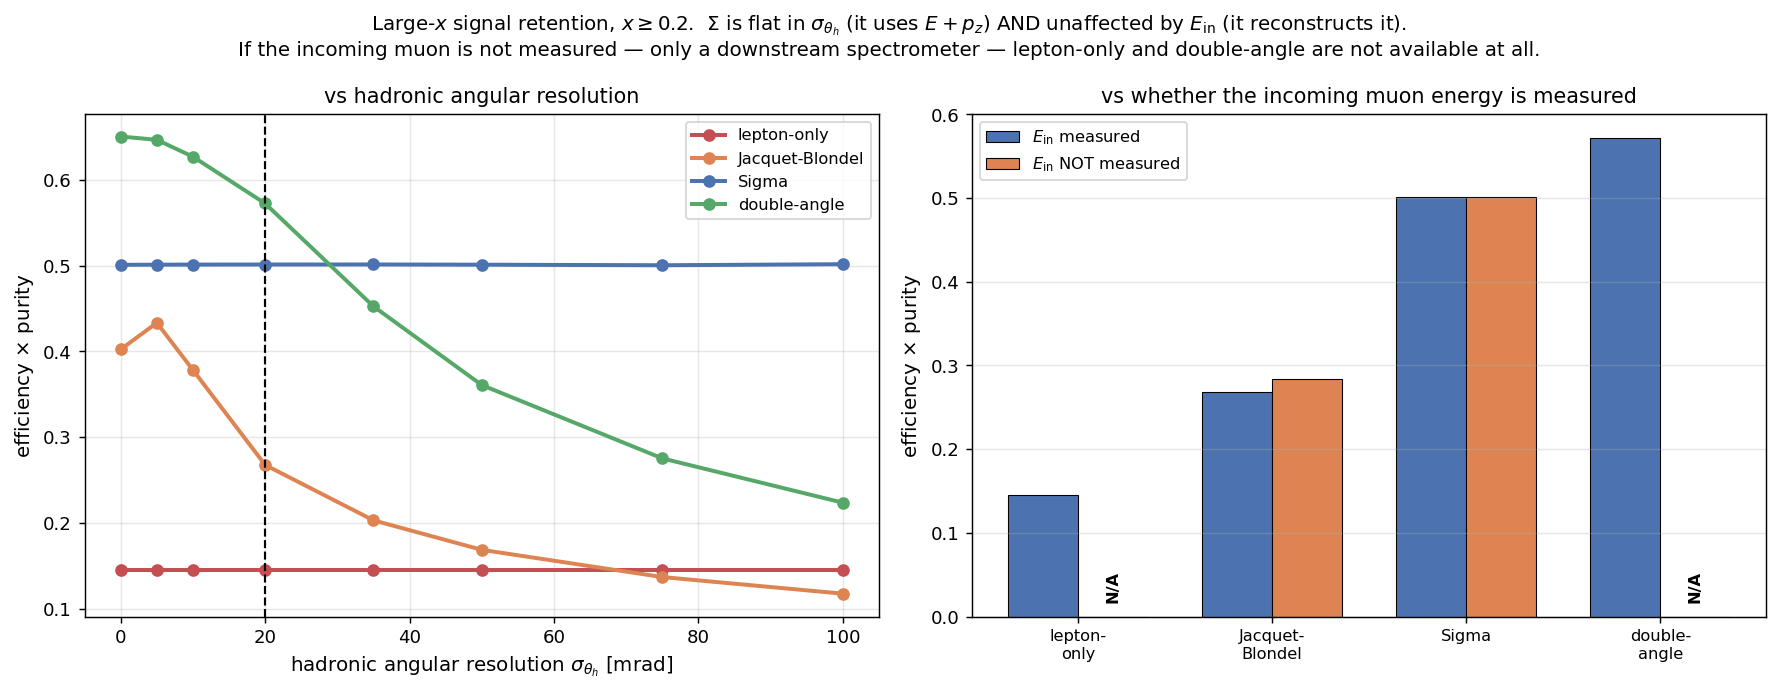
\includegraphics[width=\textwidth]{../docs/figures/31_effpur.png}
\caption{Left: signal retention versus the hadronic angular resolution. $\Sigma$
is flat; double-angle degrades steeply. Right: versus whether the incoming muon
energy is measured --- lepton-only and double-angle do not exist without it.}
\label{fig:effpur}
\end{figure}


%======================================================================
\section{Is $A_c(x)$ measurable at large $x$? No --- and not for statistical reasons}
\label{sec:acx}

Section~\ref{sec:asym} showed that $A_c$ integrated over $x$ is zero in the
available PDF sets. That is however not the end of the theoretical story:
\emph{meson-cloud} models, in which the proton fluctuates to
$|\Lambda_c^+ \bar{D}^0\rangle$ rather than to a minimal five-quark state, do
predict $c(x)\neq\bar{c}(x)$. The $c$ ends up in the baryon and the $\bar{c}$ in
the meson; their different masses give different momentum fractions. This is the
mechanism behind the recently proposed $D^+/D^-$ asymmetry
observable~\cite{lykasov}.

\paragraph{The predicted signal.} Using the Pumplin--Lai--Tung meson-cloudy-bag
parametrisation employed in Ref.~\cite{lykasov},
$f_c(x)\propto x^{1.897}(1-x)^{6.095}$ and
$f_{\bar c}(x)\propto x^{2.5}(1-x)^{4.929}$, normalised by the quark-number sum
rule, and diluting by the symmetric perturbative charm using our own
fitted/perturbative ratios:

\begin{center}\small
\begin{tabular}{lrrrrr}
\toprule
$x$ & 0.25 & 0.35 & 0.45 & 0.55 & 0.70 \\
\midrule
$A_{\rm IC}(x)$ & $+0.129$ & $-0.055$ & $-0.224$ & $-0.384$ & $-0.613$ \\
IC fraction & 0.58 & 0.76 & 0.87 & 0.93 & 0.98 \\
\textbf{observable $A(x)$} & $+0.075$ & $-0.042$ & $-0.196$ & $-0.359$ & $-0.600$ \\
\bottomrule
\end{tabular}
\end{center}

\noindent
The asymmetry \textbf{changes sign at $x=0.318$} and reaches $-0.6$ at $x=0.7$.
Two things follow immediately. First, this \emph{explains} the null result of
Sec.~\ref{sec:asym} rather than contradicting it: integrated over $x$ the
asymmetry cancels by construction (the sum rule $\int(c-\bar{c})dx=0$), so an
inclusive $A_c\approx0$ is exactly what the theory predicts. Second, at
$x\gtrsim0.5$ the predicted signal ($-0.36$ to $-0.60$) is 5--10 times larger
than the fragmentation-induced background of Sec.~\ref{sec:asym} ($-0.06$), so
the signal-to-background in the large-$x$ bins would be favourable.

\paragraph{But the tag and the signal region are kinematically incompatible.}
We therefore evaluated the tagged yield differentially in $x$. The result is
unambiguous and does not depend on any statistical argument:

\begin{table}[htbp]
\centering\small
\begin{tabular}{lrrrrr}
\toprule
True $x$ & Charm events & with semilept.\ $\mu$ & punch through & \textbf{accepted} & acceptance \\
\midrule
$0.00$--$0.05$ & 140\,057 & 25\,483 & 21\,929 & 6\,169 & $4.40\%$ \\
$0.05$--$0.10$ & 10\,530 & 1\,797 & 1\,148 & 38 & $0.36\%$ \\
$0.10$--$0.20$ & 6\,942 & 1\,140 & 558 & 5 & $0.07\%$ \\
$0.20$--$0.32$ & 4\,583 & 726 & 285 & 1 & $0.02\%$ \\
$0.32$--$0.50$ & 2\,684 & 401 & 165 & \textbf{0} & $\mathbf{0.00\%}$ \\
$0.50$--$1.00$ & 299 & 51 & 28 & \textbf{0} & $\mathbf{0.00\%}$ \\
\bottomrule
\end{tabular}
\caption{Raw Monte Carlo counts through the charm tag, versus true $\xB$
(25 seeds, $1.9\times10^6$ events). Of 6\,213 events passing the full tag,
\textbf{not one} has $\xB\geq0.32$.}
\label{tab:acceptance}
\end{table}

The mechanism is simple. Large $\xB$ means small $\nu$ at fixed $Q^2$, so the
hadronic system --- and hence the charm --- is produced with little energy. The
semileptonic decay muon is correspondingly soft and wide-angle:
\begin{center}\small
\begin{tabular}{lrr}
\toprule
& $\xB<0.1$ & $\xB\geq0.32$ \\
\midrule
decay-muon median $p$ & $13.1\GeV$ & $1.9\GeV$ \\
decay-muon median $\theta$ & $29\,$mrad & $257\,$mrad \\
\midrule
\multicolumn{3}{c}{spectrometer acceptance cone: $9.9\,$mrad} \\
\bottomrule
\end{tabular}
\end{center}
A $257\,$mrad muon cannot enter a $9.9\,$mrad cone. \textbf{The dimuon charm
charge-tag and the large-$\xB$ signal region are mutually exclusive.}

\paragraph{Consequence.} A dedicated production with an artificially asymmetric
charm PDF was considered and \textbf{not} performed: it would change the
generated $c/\bar{c}$ content but not the acceptance, so the tagged yield above
$x=0.32$ would remain zero. The handful of events reconstructed at large
$x_{\rm reco}$ (5--9 raw MC events per bin) are migrated low-$x$ events --- their
median \emph{true} $\xB$ is $0.01$ --- carrying no asymmetry.

\paragraph{What this does and does not kill.}
\begin{itemize}
  \item \textbf{$A_c(x)$ at large $x$ is not measurable} with the dimuon tag in
        this configuration. Measuring it requires a charm tag that does not
        demand the decay muon in the spectrometer.
  \item \textbf{The large-$x$ charm \emph{rate} measurement is unaffected.} It
        needs no charge information, hence no decay muon in the spectrometer,
        and it is the subject of Sec.~\ref{sec:xreco}. That result stands.
  \item The natural alternative for large-$x$ charm is the
        \textbf{charm-to-hadrons} channel, which the FASER\emph{Cal} ML tagger
        already addresses ($21\%$ efficiency at $82\%$ purity for $c\to H$ in
        neutrino events). It gives no charge information --- so it can measure
        the large-$x$ excess but not the asymmetry.
\end{itemize}

%======================================================================
\section{Systematic uncertainties --- NOT included}
\label{sec:syst}

\note{Every number in this note is a statistical or detector-resolution effect.
No systematic uncertainty is included anywhere.} This section lists what is
missing, with an estimate where one can be made cheaply.

\subsection{What was varied, and what it does}
\begin{table}[htbp]
\centering\small
\begin{tabular}{lrrr}
\toprule
Variation & $\Sigma$ & double-angle & lepton-only \\
\midrule
nominal & $0.444$ & $0.506$ & $0.151$ \\
hadronic resolution $9\%\to15\%$ & $0.442$ & $0.506$ & $0.151$ \\
hadronic resolution $9\%\to5\%$ & $0.444$ & $0.506$ & $0.151$ \\
muon resolution $\times1.3$ & $0.378$ & $0.456$ & $0.131$ \\
muon resolution $\times0.8$ & $0.521$ & $0.561$ & $0.175$ \\
hadronic angle $20\to50\,$mrad & $0.444$ & $0.356$ & $0.151$ \\
no neutrino subtraction & $0.433$ & $0.506$ & $0.151$ \\
\bottomrule
\end{tabular}
\caption{Sensitivity of the figure of merit to the modelled resolutions.}
\label{tab:syst}
\end{table}

The dominant sensitivity is to the \textbf{muon momentum resolution}, even for
the calorimetric methods --- because although $\nu$ is calorimetric, $Q^2$ still
uses the muon. The hadronic \emph{energy} resolution is essentially irrelevant
over $5$--$15\%$. The hadronic \emph{angular} resolution matters only for
double-angle.

\subsection{An actionable consequence: tracker granularity}
The CDR quotes the effect of finer SciFi granularity. Scaling to our momentum:
\begin{center}\small
\begin{tabular}{lrrrr}
\toprule
SciFi pitch & $\sigma_p/p$ at $469\GeV$ & $\Sigma$ & double-angle & $\Sigma$ AND DA \\
\midrule
$100\,\mu$m (baseline) & $38\%$ & $0.444$ & $0.506$ & $0.568$ \\
$70\,\mu$m & $29\%$ & $0.538$ & $0.572$ & $0.635$ \\
$50\,\mu$m & $26\%$ & $0.570$ & $0.605$ & $0.658$ \\
\bottomrule
\end{tabular}
\end{center}
\textbf{Going from $100$ to $50\,\mu$m improves the combined selection by
$16\%$.} Since the muon resolution is the dominant lever, this is the single
most effective detector change for this measurement.

\subsection{Systematics not evaluated at all}
\begin{enumerate}
  \item \textbf{PDF and QCD-scale uncertainties.} The LHE files carry
        \texttt{rep001--rep103} NNPDF4.0 replica and scale weights, but only the
        nominal weight is read; the replicas are discarded at both the parsing
        and showering stages. \emph{No PDF error band exists anywhere in this
        note.} For the fitted-vs-perturbative comparison this matters most,
        since the charm PDF at large $x$ is precisely the poorly-known quantity.
  \item \textbf{Absolute flux normalisation.} A residual factor $\sim1.7$
        discrepancy with Ref.~\cite{francener} remains unexplained after
        correcting the reference target mass. $F_{\rm optics}=2.0$ is the CDR's
        own estimate for a 2024 configuration, not Run 4, and the CDR states it
        is unclear whether the increase can be mitigated. $F_{\rm flux}=0.96$
        assumes the FLUKA $x$ convention matches the FASER\emph{Cal} one.
  \item \textbf{Energy scale.} Only resolutions were varied, never a
        \emph{bias}. A hadronic energy scale offset propagates directly into
        $\nu$ and hence $\xB$, and on a steeply falling spectrum a few-percent
        scale error can move the $\xB\geq0.2$ yield substantially. This should
        be evaluated.
  \item \textbf{Hadronisation model.} The $\Lambda_c/\bar{\Lambda}_c=6.8$
        leading-baryon effect, which drives the fragmentation asymmetry of
        Sec.~\ref{sec:asym}, is Pythia-specific and is not varied.
  \item \textbf{Nuclear effects.} Free-nucleon PDFs are used; no nuclear
        modification is applied for carbon or tungsten.
  \item \textbf{Detector modelling.} No reconstruction simulation: no voxel
        clustering, no shower overlap, no pile-up from the $\sim1$\,Hz/cm$^2$
        muon background, and no $\pi/K$ decay-in-flight background to the soft
        second muon.
  \item \textbf{The hadronic angular resolution} $\sigma_{\thh}=20\,$mrad has no
        documented source.
\end{enumerate}

\subsection{Statistical limitations}
The perturbative sample above $\xB=0.2$ has $N_{\rm eff}=7$. Any statement
involving the perturbative \emph{yield} or a fitted/perturbative \emph{ratio}
above $\xB=0.2$ is statistics-limited. The efficiency and purity numbers, which
use only the fitted sample ($7566$ raw events above the cut, $N_{\rm eff}=5319$),
are not affected.

%======================================================================
\section{A methodological problem worth recording}
\label{sec:hadsys}

The hadronic four-vector is computed from momentum conservation
(Eq.~\ref{eq:hadcons}), \emph{not} by summing Pythia final-state particles. The
particle sum is contaminated: the muon flux is implemented as a beam PDF of a
fictitious $7\,\mathrm{TeV}$ beam, and that beam's remnant deposits a few GeV of hadronic
activity that is not part of the DIS vertex. Energy conservation
$\Ein+M-\Eout-\Ehad\geq0$ fails in $80\%$ of events, rising to $98\%$ on the
$\xB\geq0.2$ charm sample where $\Ehad/\nu$ reaches $2.5$. It is negligible at
large $\nu$ ($\Ehad/\nu=1.02$ above $500\GeV$) but dominates exactly where the
physics is.

Three particle-level fixes were tried and all failed: dropping beam-remnant
particles (their hadronic \emph{descendants} remain); a forward-cone cut (moves
the mean, not the median); and requiring mother-chain ancestry to reach the
target beam (\emph{worse}, $\Ehad/\nu=8.5$, because Pythia's colour reconnection
leaves the ancestry graph too connected to separate the two beam sides). Using
conservation is exact and makes the closure exact by construction.

The cost is that neutrino losses must be added back explicitly, which is done:
neutrinos from charm semileptonic decays are nonzero in $35\%$ of charm events
and carry a median $13.2\GeV$ ($8.4\%$ of $\nu$) when present. Their effect is
$-10\%$ on JB and negligible on $\Sigma$.

%======================================================================
\section{Summary}

\begin{table}[htbp]
\centering\small
\begin{tabular}{p{6.3cm}p{8.6cm}}
\toprule
Question & Answer \\
\midrule
How many tagged charm events? &
$599$ charge-signed, vertex-linked charm muons in the 3DCal
($4058$ including the AHCAL) at $780\fb$. \\[3pt]
Is charm/anticharm separable? &
Yes in principle --- the decay-muon charge \emph{is} the charm sign, and the CDR
spectrometer misidentifies $<0.7\%$ --- but the reach is
$\sigma(A_c)=0.041$. \\[3pt]
Is $A_c$ an intrinsic-charm observable? &
\textbf{No.} It is identically zero in both available PDF sets. A non-zero
$A_c$ needs a PDF set with explicit charm asymmetry, or a model. A
fragmentation-induced asymmetry of the same size as our reach competes with
it. \\[3pt]
What is the accessible IC signal? &
The large-$\xB$ charm excess: $\times1.8$ at $\xB=0.2$ rising to $\times44$ at
$0.7$. Above $\xB=0.2$ the charm is $\approx99\%$ IC-attributable. \\[3pt]
Does muon smearing destroy it? &
For lepton-only, \textbf{yes} --- $\nu$ is $7.7\%$ of $\Ein$, so $38\%$ muon
resolution gives a several-hundred-percent $\nu$ error and no correlation
between $x_{\rm true}$ and $x_{\rm reco}$. \\[3pt]
Do calorimetric methods rescue it? &
\textbf{Yes.} $\Sigma$ retains $\times2.9$ more signal; $\Sigma$ AND
double-angle $\times3.8$, lifting the IC purity of the selection from $64\%$ to
$95\%$. \\[3pt]
Which method should be used? &
\textbf{$\Sigma$}, combined with double-angle where possible. $\Sigma$ is flat in
the hadronic angular resolution, unaffected by the neutrino loss, and the only
method that works when $\Ein$ is unmeasured. \\[3pt]
Do neutral particles undermine it? &
No. Neutrinos cost JB $10\%$ and $\Sigma$ nothing; neutral hadrons are $8\%$ of
the visible energy. \\[3pt]
What most improves the measurement? &
The \textbf{muon momentum resolution}. Going from $100$ to $50\,\mu$m SciFi
pitch improves the combined selection by $16\%$. \\[3pt]
Is $A_c(x)$ measurable at large $x$? &
\textbf{No}, and for a kinematic not a statistical reason: of 6213 tagged MC
events, none has $\xB\geq0.32$. Large $\xB$ implies small $\nu$, hence a soft
($1.9\GeV$) wide-angle ($257\,$mrad) decay muon that cannot enter the $9.9\,$mrad
spectrometer cone. The tag and the signal region are mutually exclusive
(Sec.~\ref{sec:acx}). \\[3pt]
Are systematics included? &
\note{No. Nothing in this note includes a systematic uncertainty}
(Sec.~\ref{sec:syst}). PDF uncertainties in particular are entirely absent,
although the replica weights exist in the LHE files. \\
\bottomrule
\end{tabular}
\caption{Summary of findings.}
\end{table}

\section*{Next steps}
\begin{enumerate}
  \item Evaluate PDF and scale uncertainties using the \texttt{rep001--rep103}
        weights, which requires carrying them through the showering step.
  \item Evaluate energy-\emph{scale} systematics, not just resolutions.
  \item Replace $\sigma_{\thh}=20\,$mrad with a value from the FASER\emph{Cal}
        reconstruction.
  \item Implement a constrained kinematic fit (cf.\ Ref.~\cite{francener}
        Sec.~4.2) in place of the crude AND of two cuts.
  \item Generate a high-statistics perturbative-charm sample so that
        fitted/perturbative ratios above $\xB=0.2$ become meaningful.
  \item Simulate the $\pi/K$ decay-in-flight background to the soft second muon.
\end{enumerate}

\begin{thebibliography}{9}
\bibitem{francener} R.~Francener \emph{et al.},
  ``Deep-Inelastic Scattering at TeV Energies with LHC Muons'',
  \href{https://arxiv.org/abs/2506.13889}{arXiv:2506.13889}.
\bibitem{cdr} FASER\emph{Cal} Collaboration,
  ``The FASERCal Conceptual Design Report'', CERN-FASER-NOTE-2026-004, v0,
  16 February 2026.
\bibitem{talk} ``FASERCal'', FASER Collaboration Meeting, Bern, 15 July 2026.
\bibitem{lykasov} G.~I.~Lykasov, A.~A.~Sorokovikov and S.~J.~Brodsky,
  ``Intrinsic charm and the $D^+$--$D^-$ asymmetry produced in proton-proton
  collisions'', Phys.\ Rev.\ D \textbf{111} (2025) 074035,
  \href{https://arxiv.org/abs/2501.02507}{arXiv:2501.02507}.
  Parametrisation originally from J.~Pumplin, H.~L.~Lai and W.~K.~Tung,
  Phys.\ Rev.\ D \textbf{75} (2007) 054029.
\bibitem{bassler} U.~Bassler and G.~Bernardi,
  ``On the kinematic reconstruction of deep inelastic scattering at HERA:
  the $\Sigma$ method'', Nucl.\ Instrum.\ Meth.\ A \textbf{361} (1995) 197.
\end{thebibliography}

\end{document}
